\chapter*{Introduzione}
\addcontentsline{toc}{chapter}{Introduzione}

\chapter{Probabilità e meccanica statistica}
In questo capitolo vengono introdotti alcuni concetti fondamentali di probabilità necessari per comprendere il problema del campionamento: esso consiste nel generare una successione di configurazioni secondo una determinata distribuzione di probabilità. Tale problema assume particolare rilevanza in meccanica statistica, dove le proprietà macroscopiche di un sistema possono essere ricavate a partire dalle configurazioni microscopiche che lo costituiscono.

Dopo aver introdotto le nozioni di base relative alle variabili aleatorie e alle distribuzioni di probabilità, si discuterà l'importanza del campionamento di una distribuzione. Infine, si introdurrà l'ensemble canonico, con particolare attenzione alla distribuzione di Boltzmann, che rappresenta la distribuzione target dei metodi di campionamento studiati nel seguito di questa tesi.

\section{Teoria della probabilità}
\subsection{Spazi di probabilità e variabili aleatorie}
In teoria della probabilità ha un ruolo fondamentale \textbf{lo spazio di probabilità} ($ \Omega, P$): dove $\Omega$ è l'insieme di tutti i possibili eventi $\chi$ e $P$ è una misura di probabilità su $\Omega$. Un sottoinsieme $A \subset \Omega$ è chiamato evento ed ad ogni evento è possibile associare un numero reale $P(A) \in [0, 1]$ - ovvero la probabilità di tale evento. In particolare è necessario che sia soddisfatte $P(\Omega) = 1$, $ P(\emptyset) = 0$ e per ogni insieme di eventi disgiunti $A_1, A_2,  ...$ vale:

\begin{equation}
    P(A_1 \cup A_2 \ ...) = P(A_1) + P(A_2) + ...
\end{equation}

\begin{example}{Tiri di un dado}{dice}
Quando si tira un dado a sei facce si considera lo spazio degli eventi $\Omega = \{1, 2, ... , 6\}$ e la misura di probabilità $P({\chi_i}) = 1/6$ per ogni $\chi_i \in \Omega$ .
Un esempio di evento è il caso in cui risultato del tiro sia pari $A =\{2, 4, 6\} \subset \Omega$ con probabilià calcolabile nel seguente modo: $P(A) = P({1}) + P({2}) + P({3}) = 1/2$.
\end{example}


Una \textbf{variabile aleatoria} (reale) $X$ che associa agli elementi di uno spazio degli esiti $\Omega$ valori appartenenti a uno spazio misurabile $(\mathbb{R})$. 
Una variabile aleatoria $X$ associa a ciascun esito $\chi$ un valore $x$ appartenente allo spazio dei valori possibili della variabile. Nel caso di una variabile aleatoria reale si ha quindi:
\begin{equation}
X:\Omega \rightarrow \mathbb{R}.
\end{equation}

\subsection{Distribuzioni di probabilità continue}

La distribuzione di probabilità associata a una variabile aleatoria continua $X$ è descritta da una densità di probabilità $p_X(x)$, che determina come la probabilità è distribuita nello spazio dei possibili valori di $X$. La densità di probabilità deve soddisfare la condizione di normalizzazione
\begin{equation}
\int_{-\infty}^{+\infty}p_X(x) \ dx=1.
\end{equation}

È importante sottolineare che, nel caso continuo, la densità di probabilità non rappresenta direttamente la probabilità che la variabile assuma un determinato valore. Infatti, la probabilità di ottenere esattamente un particolare valore $x_0$ è nulla. La densità di probabilità permette invece di calcolare la probabilità che la variabile aleatoria assuma un valore appartenente a un determinato intervallo. In particolare, la probabilità che $X$ appartenga all'intervallo $[a,b]$ è data da
\begin{equation}
P(a\leq X\leq b)
=
\int_a^b p_X(x) dx.
\end{equation}

La distribuzione di probabilità può quindi essere interpretata geometricamente: la probabilità associata a un intervallo corrisponde all'area sottesa dalla densità di probabilità nell'intervallo considerato. Una maggiore densità di probabilità in una determinata regione indica quindi una maggiore probabilità di osservare valori della variabile in quella regione.

Nel seguito sarà particolarmente utile considerare variabili aleatorie multidimensionali. Una configurazione microscopica di un sistema fisico può infatti essere rappresentata mediante un vettore
\begin{equation}
\mathbf{x}=(x_1,x_2,\ldots,x_D)\in\mathbb{R}^D,
\end{equation}
dove $D$ rappresenta il numero di gradi di libertà del sistema. In questo caso la distribuzione di probabilità è descritta da una densità $p(\mathbf{x})$, normalizzata secondo
\begin{equation}
\int_{\mathbb{R}^D}p(\mathbf{x})d\mathbf{x}=1.
\end{equation}

La densità $p(\mathbf{x})$ permette di determinare la probabilità che una configurazione appartenga a una determinata regione $\mathcal{A}$ dello spazio delle configurazioni:
\begin{equation}
P(\mathbf{x}\in\mathcal{A})
=
\int_{\mathcal{A}}p(\mathbf{x}) \ d\mathbf{x}.
\end{equation}

Nel caso multidimensionale la probabilità è l'integrale della densità di probabilità su una regione dello spazio delle configurazioni. Analogamente al caso unidimensionale, non è la probabilità associata a una singola configurazione a essere rilevante, ma la probabilità complessiva associata a una regione dello spazio.

Una distribuzione di probabilità può inoltre presentare una struttura caratterizzata dalla presenza di uno o più massimi locali. In particolare, si definisce distribuzione \textit{unimodale} una distribuzione caratterizzata da un'unica regione di massima probabilità detta \textit{modo}. Un esempio tipico è rappresentato dalla distribuzione gaussiana, che presenta un unico massimo in corrispondenza del suo valore medio.

Una distribuzione \textit{multimodale}, invece, presenta più regioni distinte di alta probabilità, associate a più massimi locali della densità. In questo caso, ciascun massimo identifica un modo della distribuzione. Le diverse regioni ad alta probabilità possono essere separate da regioni caratterizzate da una densità molto più bassa.

\begin{figure}[H]
    \centering
    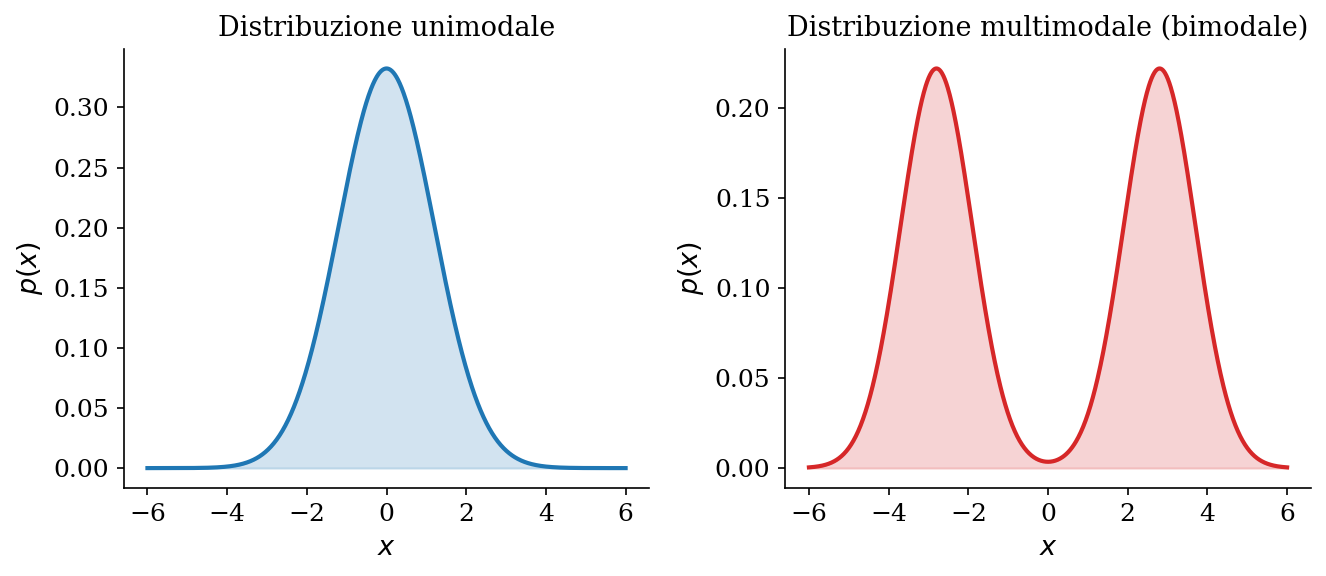
\includegraphics[width=0.9\textwidth]{images/uni_multi.png}
    \caption{Confronto tra una distribuzione unimodale (gaussiana) e una distribuzione multimodale (bimodale).}
    \label{fig:uni_multi}
\end{figure}

La distinzione tra distribuzioni unimodali e multimodali è particolarmente importante nel problema del campionamento. Nel caso di una distribuzione unimodale, un metodo di campionamento che esplori efficacemente la regione attorno al massimo della distribuzione può ottenere un campione rappresentativo dell'intera distribuzione. Nel caso multimodale, invece, il campionamento può risultare più complesso, poiché è necessario esplorare tutte le regioni rilevanti dello spazio delle configurazioni e riprodurre correttamente la probabilità associata a ciascun modo e non esclusivamente a quello di maggiore densità.

Se le diverse regioni ad alta probabilità sono separate da barriere caratterizzate da una probabilità molto bassa, un metodo di campionamento locale può infatti rimanere confinato per lungo tempo all'interno di uno dei modi, esplorando con difficoltà gli altri. Questo fenomeno rappresenta una delle principali difficoltà associate al campionamento di distribuzioni multimodali e costituisce uno degli aspetti centrali affrontati nel seguito della tesi.

\subsection{Valori di aspettazione e campionamento}

Sia $O(\mathbf{x})$ una funzione della variabile aleatoria, il valore di aspettazione è calcolabile tramite il seguente integrale:

\begin{equation}
\langle O(\mathbf{x})\rangle
=
\int_{\mathbb{R}^D} O(\mathbf{x})p(\mathbf{x}) \ d\mathbf{x}.
\end{equation}

La convergenza dell'integrale non è affatto garantita e dipende dall'andamento della funzione $O(\mathbf{x})$ e da $p(\mathbf{x})$, inoltre questo integrale non è sempre facilemente risolvibile analiticamente o numericamente.
Un approccio diretto al calcolo di $\langle O(\mathbf{x})\rangle$ potrebbe basarsi su metodi di quadratura numerica, che discretizzano lo spazio delle configurazioni su una griglia e approssimano l'integrale come somma pesata sui punti della griglia. Se lo spazio delle configurazioni ha dimensione $D$ e si utilizzano $n$ punti per ciascuna direzione, il numero totale di valutazioni della funzione integranda cresce come $n^D$. Per sistemi con un numero elevato di gradi di libertà, come tipicamente accade in meccanica statistica, questa crescita esponenziale rende i metodi di quadratura del tutto inapplicabili: questo fenomeno è noto come \textit{maledizione della dimensionalità}.

È in questo contesto che il campionamento assume un ruolo centrale. Anziché valutare la funzione integranda su una griglia deterministica, l'idea alla base dei metodi di campionamento consiste nel generare un insieme di configurazioni $\{\mathbf{x}_1,\mathbf{x}_2,\ldots,\mathbf{x}_N\}$ distribuite secondo la densità di probabilità $p(\mathbf{x})$, e nello stimare il valore di aspettazione mediante la media aritmetica
\begin{equation}
\langle O(\mathbf{x})\rangle
\approx
\overline{O}_N
=
\frac{1}{N}\sum_{i=1}^{N}O(\mathbf{x}_i).
\label{eq:mc_estimator}
\end{equation}

Per la legge dei grandi numeri, lo stimatore $\overline{O}_N$ converge, per $N\rightarrow\infty$, al valore di aspettazione esatto $\langle O(\mathbf{x})\rangle$, a patto che le configurazioni $\mathbf{x}_i$ siano effettivamente distribuite secondo $p(\mathbf{x})$. Un aspetto cruciale di questo approccio è che, se le configurazioni sono indipendenti e identicamente distribuite, l'errore statistico associato allo stimatore decresce come
\begin{equation}
\sigma_{\overline{O}_N} \sim \frac{\sigma_O}{\sqrt{N}},
\end{equation}
dove $\sigma_O$ è la deviazione standard di $O(\mathbf{x})$ rispetto a $p(\mathbf{x})$. Diversamente dai metodi di quadratura, questo risultato non dipende esplicitamente dalla dimensione $D$ dello spazio delle configurazioni: è questa caratteristica a rendere i metodi di campionamento lo strumento privilegiato per lo studio di sistemi ad alta dimensionalità. Il problema del campionamento, in questo senso, precede logicamente quello della stima delle osservabili, e sarà l'oggetto centrale dei metodi discussi nei capitoli successivi.

\section{Ensemble statistici}



\subsection{L'ensemble canonico}
Consideriamo un sistema fisico descritto da una hamiltoniana $\mathcal{H}(\mathbf{x})$ dove $\mathbf{x}$
rappresenta collettivamente i gradi di libertà del sistema: posizioni, impulsi, o in generale le variabili che definiscono uno stato microscopico. L'ensemble canonico permette di descrivere il comportamento termodinamico di un sistema posto a contatto termico con un \textit{reservoir}  a temperatura $T$ fissata, con cui può scambiare energia ma non particelle. L'energia del sistema fluttua attorno a un valore medio $\langle E \rangle$ determinato dall'equilibrio termico con il serbatoio.

\subsection{La distribuzione di Boltzmann}


Il comportamento del sistema a fissata $T$ è descritto da una distribuzione di probabilità $\rho (\mathbf{x}, T)$ ottenibile attraverso il principio di massima entropia.
\begin{equation}
    \mathcal{S} = - \int_{\mathbb{R}^D} \rho (\mathbf{x}, T) \ln(\rho(\mathbf{x}, T)) d\mathbf{x}
\end{equation}

Per massimizzare l'entropia si utilizza il teorema dei moltiplicatori di Lagrange:

\begin{equation}
    \mathcal{L}[\rho] = -\int_{\mathbb{R}^D} \rho \ln \rho \, d\mathbf{x} - \alpha \left( \int_{\mathbb{R}^D} \rho \, d\mathbf{x} - 1 \right) - \beta \left( \int_{\mathbb{R}^D} \rho \, \mathcal{H} \, d\mathbf{x} - \langle E \rangle \right),
\end{equation}

dove $\alpha$ e $\beta$ sono i moltiplicatori di Lagrange associati rispettivamente al vincolo di normalizzazione

\begin{equation}
    \int_{\mathbb{R}^D} \rho(\mathbf{x}, T) \ d\mathbf{x} = 1
\end{equation}

e al vincolo sul valore medio dell'energia

\begin{equation}
    \int_{\mathbb{R}^D} \rho(\mathbf{x}, T) \, \mathcal{H}(\mathbf{x}) \, d\mathbf{x} = \langle E \rangle .
\end{equation}

La massimizzazione impone $\delta \mathcal{L}/\delta \rho = 0$ restituendo:

\begin{equation}
    -\ln\rho(\mathbf{x}, T) - 1 - \alpha - \beta \mathcal{H}(\mathbf{x}) = 0
\end{equation}

che permette di determinare $\rho (\mathbf{x}, T)$:

\begin{equation}
    \rho(\mathbf{x}, T) = e^{-1-\alpha} \, e^{-\beta \mathcal{H}(\mathbf{x})}.
\end{equation}

Il moltiplicatore $\alpha$ è fissato dalla condizione di normalizzazione: definendo la \textit{funzione di partizione}

\begin{equation}
    Z(\beta) = \int_{\mathbb{R}^D} e^{-\beta \mathcal{H}(\mathbf{x})} \ d\mathbf{x},
\end{equation}

si ha $e^{-1-\alpha} = 1/Z(\beta)$, da cui \textit{la distribuzione di Boltzmann}:

\begin{equation}
    \rho(\mathbf{x}, T) = \frac{1}{Z(\beta)} e^{-\beta \mathcal{H}(\mathbf{x})}.
\end{equation}

Dove è $\beta = 1/(k_B T)$.

Nota sul fatto che Z è un integrale multidimensionale e quindi non è sempre calcolabile e di conseguenza non è possibile calcolare il valore della distribuzione, dunque si utilizza il metodo del campionamento.....